\fancychapter{Evaluation Metrics}

\section{Clustering Tweets with Self-Organizing Maps}
\label{ch:clustering_tweets}

\subsection{Twitter Dataset}
\label{subsec:twitter_dataset}

As can be seen in Figure~\ref{fig:json_tweet_user} no information about the social relations of the user which emitted the tweet are present. Therefor in order to retrieve the social network in which a user is contained, it will be necessary to connect to the Twitter API. Crawling twitter is discussed in further depth in Chapter~\ref{chap:crawling_twitter}.  


In order to better understand the dataset at hand, all the \ac{JSON} files where converted into \ac{CSV}in a way to reduce the size of the dataset. While tweets where being converted, \ac{URL} where removed --- since most of them where minified in order to fit in less that 140 characters, without translating the minified URL, not a lot of information can be gathered. Also, all tweets that where not identified as being in English where also removed. The tweet shown in \ac{JSON} format in Figure~\ref{fig:json_tweet} is converted to \ac{CSV} in Figure~\ref{fig:csv_tweet}.

\begin{figure}
  \begin{center}
    \begin{lstlisting}[language=json,firstnumber=1]
    karmadabaghi,A Paintbrush That Works On The iPad @sensubrushman
    \end{lstlisting}
  \end{center}
  \caption{\ac{CSV} representation of a Tweet. The username is present in the first column and the tweet text on the last.}
  \label{fig:csv_tweet}
\end{figure}


{\color{red} Add table with dataset characteristics }
%\begin{tabular}{c | c}
  %Number of Files  & 337\\
  %Average File Size  & 337\\
%\end{tabulartabular}


\subsection{SOM training}
\label{sub:clustering_tweets_with_soms}
{\color{red} Refer dataset info on }
{\color{red} Describe naive approach to SOM training in R }
{\color{red} Describe amount of weird words }

\subsection{Reducing SOM vector size}
\label{sub:reducing_som_vector_size}
In Subsection~\ref{sub:clustering_tweets} we introduced string reducer methods which enabled great \ac{VSM} reduction. On Figure~\ref{fig:plot_word_red} we can see the amount of words removed by each method alone, and by all methods combined --- column "All Methods"---. In order to build this graph, we applied each method independently to a sample of 902802 tweets.

\begin{figure}[htpb]
  \centering
  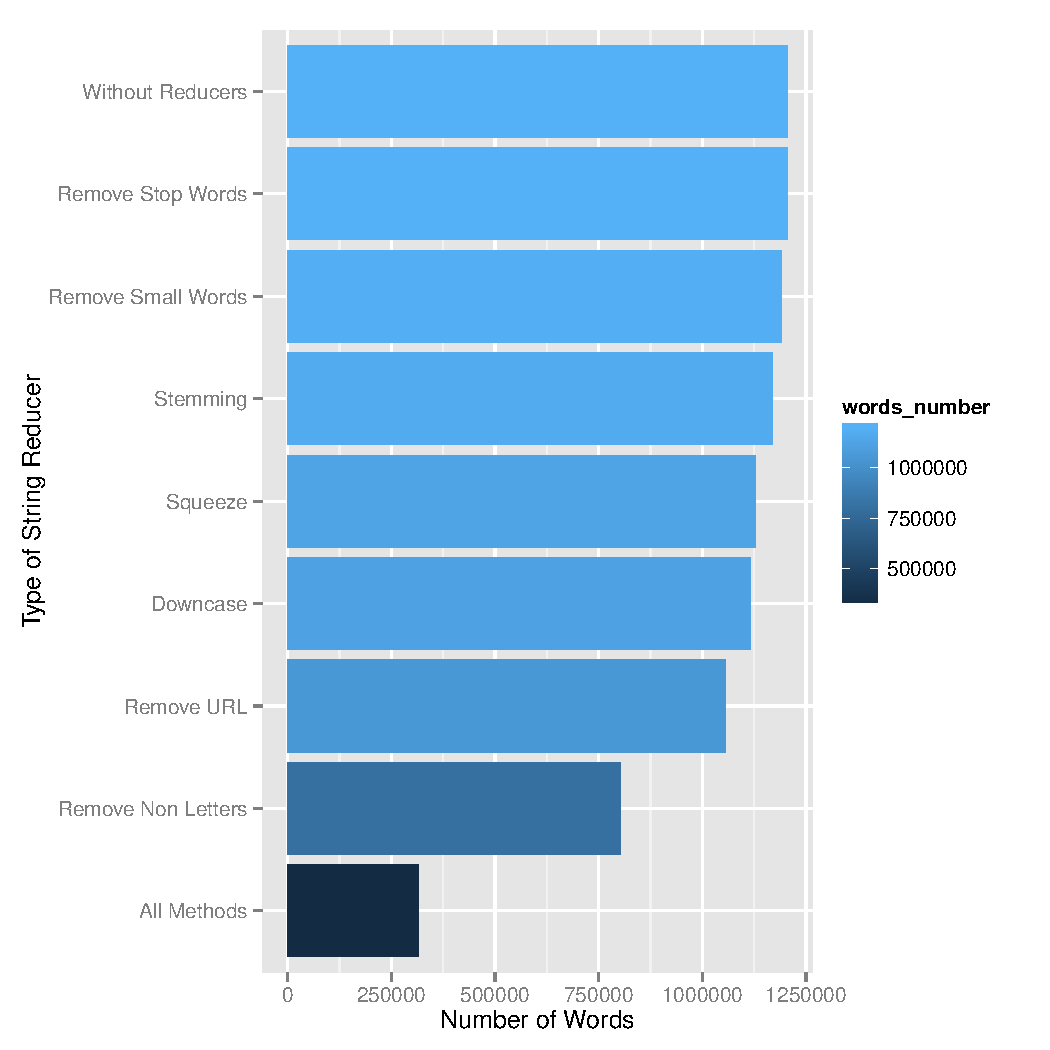
\includegraphics[width=0.8\linewidth]{./plots/svm/plot_wordcount.pdf}
  \caption{Amount of unique words present on dataset sample with 902802, based on the string word reduction technique applied.}
  \label{fig:plot_word_red}
\end{figure}

It is interesting to see that each method by itself doesn't remove a great amount of words. The method that removed more words by itself was "remove non letters" --- which removes every character that is not a letter ---, at an order of 33\%. On the other hand, the method "remove stop words" by itself removed only 400 of words. This was expected due to the fact that the full list of MySQL stop words used by this method only has 543 words. All methods combined where able to reduce the \ac{VSM} size in about 75\%.

String reduction techniques work directly with text and has no notion whatsoever of linguistic semantics. I Subsection~\ref{sub:tweeter_natural_language_processing} we presented a twitter \ac{NLP} libray which can be used effectively to understand the linguistic semantics used on twitter. 

By feeding the same dataset as used above to the library we where able to identify multiple types of words that can afterwards be considered relevant for~\ac{TDT}. On Figure \ref{fig:plot_word_red}, the red bars show the amount of words unique words found under a specific semantic tag, whilst in red we can see words tagged under the same category after applying string reduction techniques.

Due to the fact that we are trying to identify topics, most of the tagged words are of no use. We chose to use only common nouns, proper nouns and hashtags during the clustering process. By applying all these filters to the dataset sample, we have a \ac{VSM} reduction of about 90\%, from 1 204 743 different words to 132 861.

\begin{figure}[htpb]
  \centering
  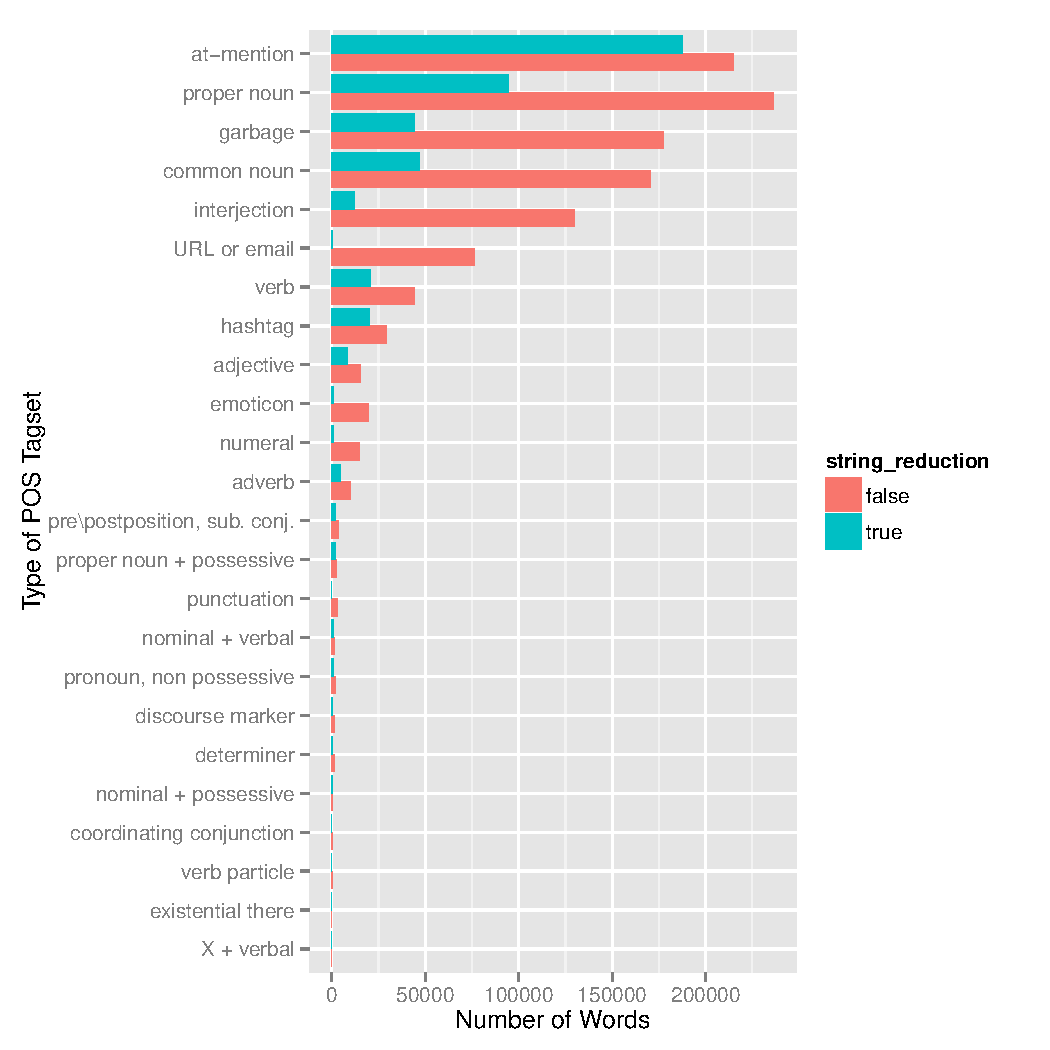
\includegraphics[width=0.8\linewidth]{./plots/svm/plot_wordcount_nlp.pdf}
  \caption{Number of words tagged with Ark Tweet NLP. In red we can see the number of words unique words tagged in each category, while in blue we can see the amount of unique words, after applying string reduction techniques.}
  \label{fig:wordcount_nlp}
\end{figure}

\subsubsection{Identify Tweets language}
\label{ssub:identify_tweets_lang}
Identifying tweets that where not in the English language was done through the usage of Ruby library called whatlanguage~\footnote{https://github.com/peterc/whatlanguage}, which tries to identify one language through Bloom Filters. Inside the tweet there is a field which identifies the user language, we found that x is not acurate. Removing tweets that weren't in the english language reduced the amount of different words in x and therefor will reduce the dimensional size of the \ac{SOM}.

\subsubsection{Text Manipulation for VSM reduction}
\label{ssub:Text Manipulation for SVM reduction}

Work done on the INESC twitter dataset with SOMs.
SOM implementations used, what where their strong points and weaknesses

\subsubsection{Clustering with Word Selection }
\label{ssub:Word Selection for Clustering}
{\color{red} Results of SOMs using selected words based on occurrence after applying SVM reduction }
{\color{red} Results where pretty bad }

\subsection{Clustering with NLP selected words}
\label{sub:clustering_with_nlp_selected_words}
{\color{red} results of som using arktweet NLP }
{\color{red} types of tags selected }
{\color{red} show tweets that had no representation }
{\color{red} review clusters and results }

\subsection{Conclusions}
\label{sub:conclusions}



\section{Twitter Crawler}
\label{sec:twitter_crawler}
  This problem could be solved in any of the following ways:
\begin{itemize}
  \item \textbf{First aproach: } For each tweet, fetch the user information including the users he is connected to.
  \item \textbf{Second aproach: } Create our own crawler, where the social connections, tweets and users are saved.
\end{itemize}                                                                                             

When designing the twitter crawler, we took into consideration that it had to be extremely resilient in order to be able to be left alone, crawling the twitter, until told to stop. Also if anything happened to the machine where the crawler was running it would be necessary to return to some previous crawling state, with minimum data loss. Algorithm {\color{red} I NEED TO WRITE THIS ALGORITHM } shows the crawler algorithm, which works in the following way:

\begin{itemize}
  \item \textbf{Step 1:} Choose some seed users to start crawling or deserialize a serialized version of the crawler if available.
  \item \textbf{Step 2:} For each seed user get all of his followers, and add them to an array if they haven't yet been crawled.
  \item \textbf{Step 3:} Repeat step one with random users taken from the array on step 2, until API limit is reached.
  \item \textbf{Step 4:} When API limit is reached, print the state of the crawled network, serialize the current state, and wait 15 minutes until it is possible to resume crawling. 
\end{itemize}

\subsection{Crawler Performance}
\label{sub:crawler_performance}
{\color{red} show number of tweets per second, number user per second, and users reached per second. }
{\color{red} compare the with the theoretical maximum }
{\color{red} compare size of the serialized social network with the amount of tweets and users it is getting  }
{\color{red} compare time taken to deserialize with amount of tweets crawled }
{\color{red} compare time to serialize with amount of tweets crawled }
 


\section{SOM Framework}
\label{sec:som_framework}
The \ac{SOM} framework was developed in the Ruby programing language \footnote{https://www.ruby-lang.org/en/} due to the desired characteristic of allowing great levels of introspection and being an almost pure object oriented programing language. Due to this characteristics making modifications to core parts of the algorithm is fairly easy.

The \ac{SOM} Framework was developed in a test driven fashion, having 100\% of its public methods tested and documented for expected behavior. These characteristics, associated with the fact that was published under an open source license, makes it available for other researchers to implement their own SOM variants.

By default, the base SOM algorithm is implemented as described by the Algorithm~\ref{alg:som} in Section \ref{sec:the_self_organizing_map}. 
\subsection{Clustering Color Vectors}
\label{sub:main_features}
Out of the box, the \ac{SOM} Framework implements a squared output space, where all residing neurons are manipulated as arrays. It is possible ate any given moment of the training to export the output space to \ac{JSON}, \ac{CSV} or to visualize its current \ac{U-Matrix}. Also during training a progress bar is displayed in order to know how much time will be needed for the training to end.

Due to the features described above, it is possible to train a \ac{SOM} to identify random colors --- RGB vectors --- while printing the results. In order to do this we will start by:
\begin{itemize}
  \item Initializing a SOM object with an output space size of 15 by 15 neurons, which will yield a total of 255 neurons --- and directly maps to the maximum number of clusters --- and 700 epochs.
  \item Create 1500 input patterns with size 3 and random values between 0 and 255. 
  \item Tell the SOM to print its state at the end of each epoch.
\end{itemize}
The machine used for training had the hardware specifications outlined in table \ref{tab:mac_test}

\begin{table}[H]
  \caption{Test machine one specs}
  \label{tab:mac_test}
  \begin{center}
    \begin{tabular}{|c|c|}
      \hline
      Operative System & OSX 10.9.5 \\
      \hline
      Memory           & 8 GB, 1067MHz DDR3       \\
      \hline
      Processor        & 2,4GHz Intel Core 2  Duo \\
      \hline
      Hard Drive       & 128GB SSD  \\
      \hline
    \end{tabular}
  \end{center}
\end{table}


A summary of the training is specified in Table~\ref{tab:som_colours}
\begin{table}[H]
  \caption{SOM trainning resumed}
  \label{tab:som_colours}
  \begin{center}
    \begin{tabular}{|c|c|}
      \hline
      \textbf{Number of Neurons} & 225 \\
      \hline
      \textbf{Output Space Size} & 15x15 \\
      \hline
      \textbf{Number of Input Patterns} & 1500 \\
      \hline
      \textbf{VSM size of Input Patterns and Neurons} & 3 \\
      \hline
      \textbf{Number of Epochs} & 600 \\
      \hline
      \textbf{Training Duration} & 14 hours \\
      \hline
      \textbf{Type of Train} & print each epoch training\\
      \hline
      \textbf{Initial learning rate} & 0.6\\
      \hline
      \textbf{Initial Radius} & 8\\
      \hline
    \end{tabular}
  \end{center}
\end{table}


\begin{figure}[h]
  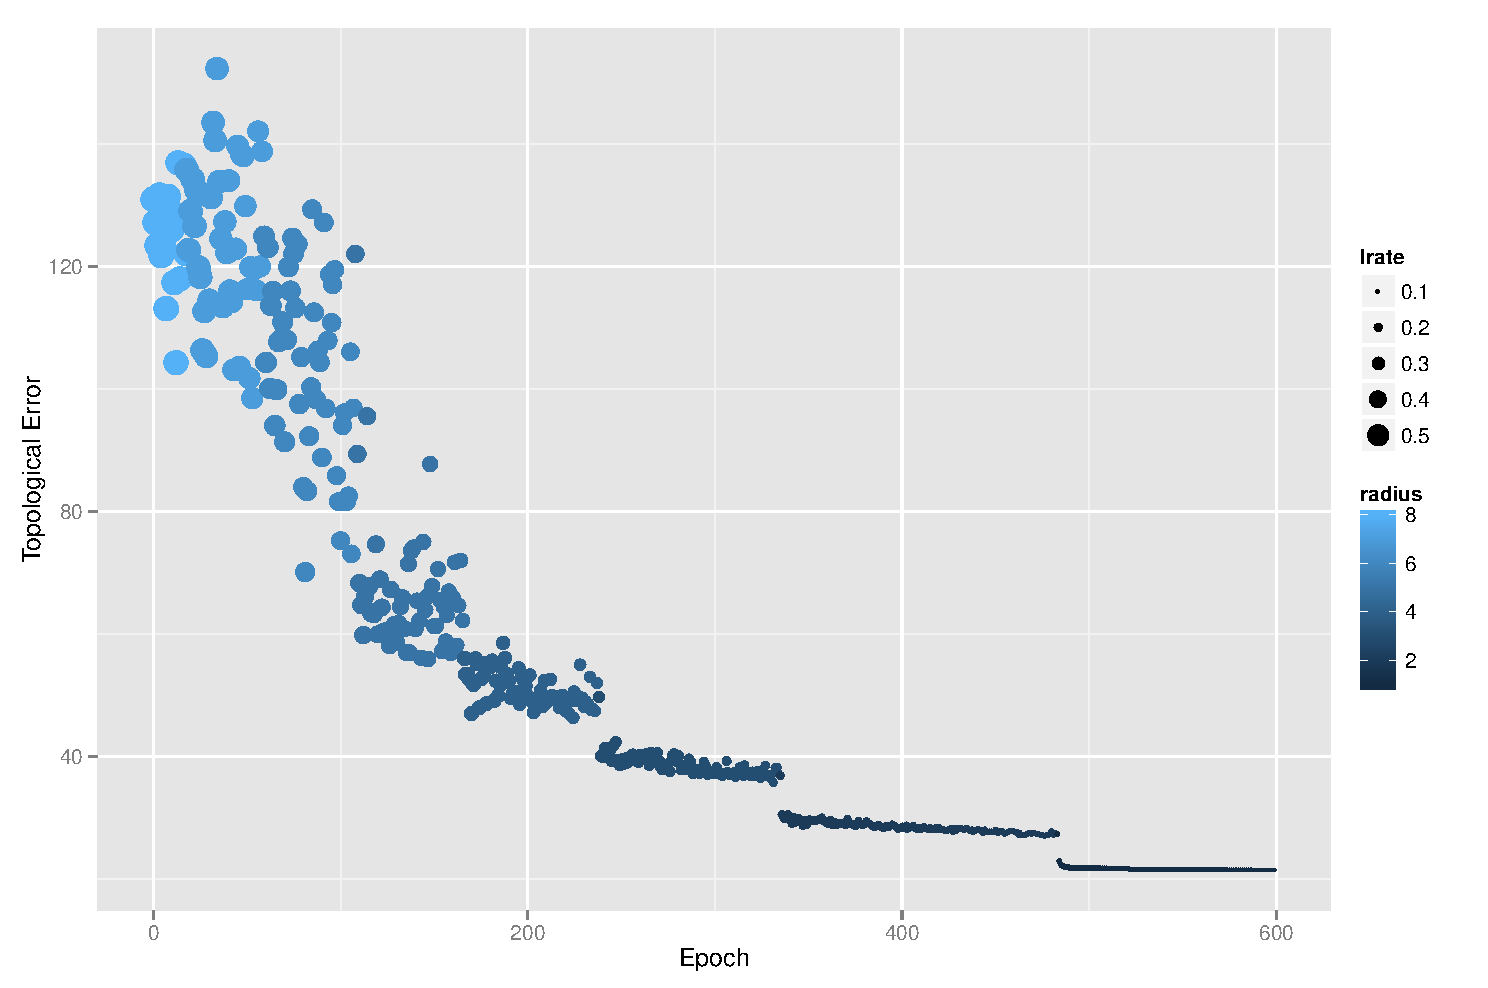
\includegraphics[scale=0.6]{./plots/som/topological_error.pdf}
  \label{fig:top_error}
  \caption{Changes in topological error throughout the SOM training, lrate stands for learning rate, and radius for radius applied to the winning neuron}
\end{figure}

\begin{figure}[h]
  \centerline{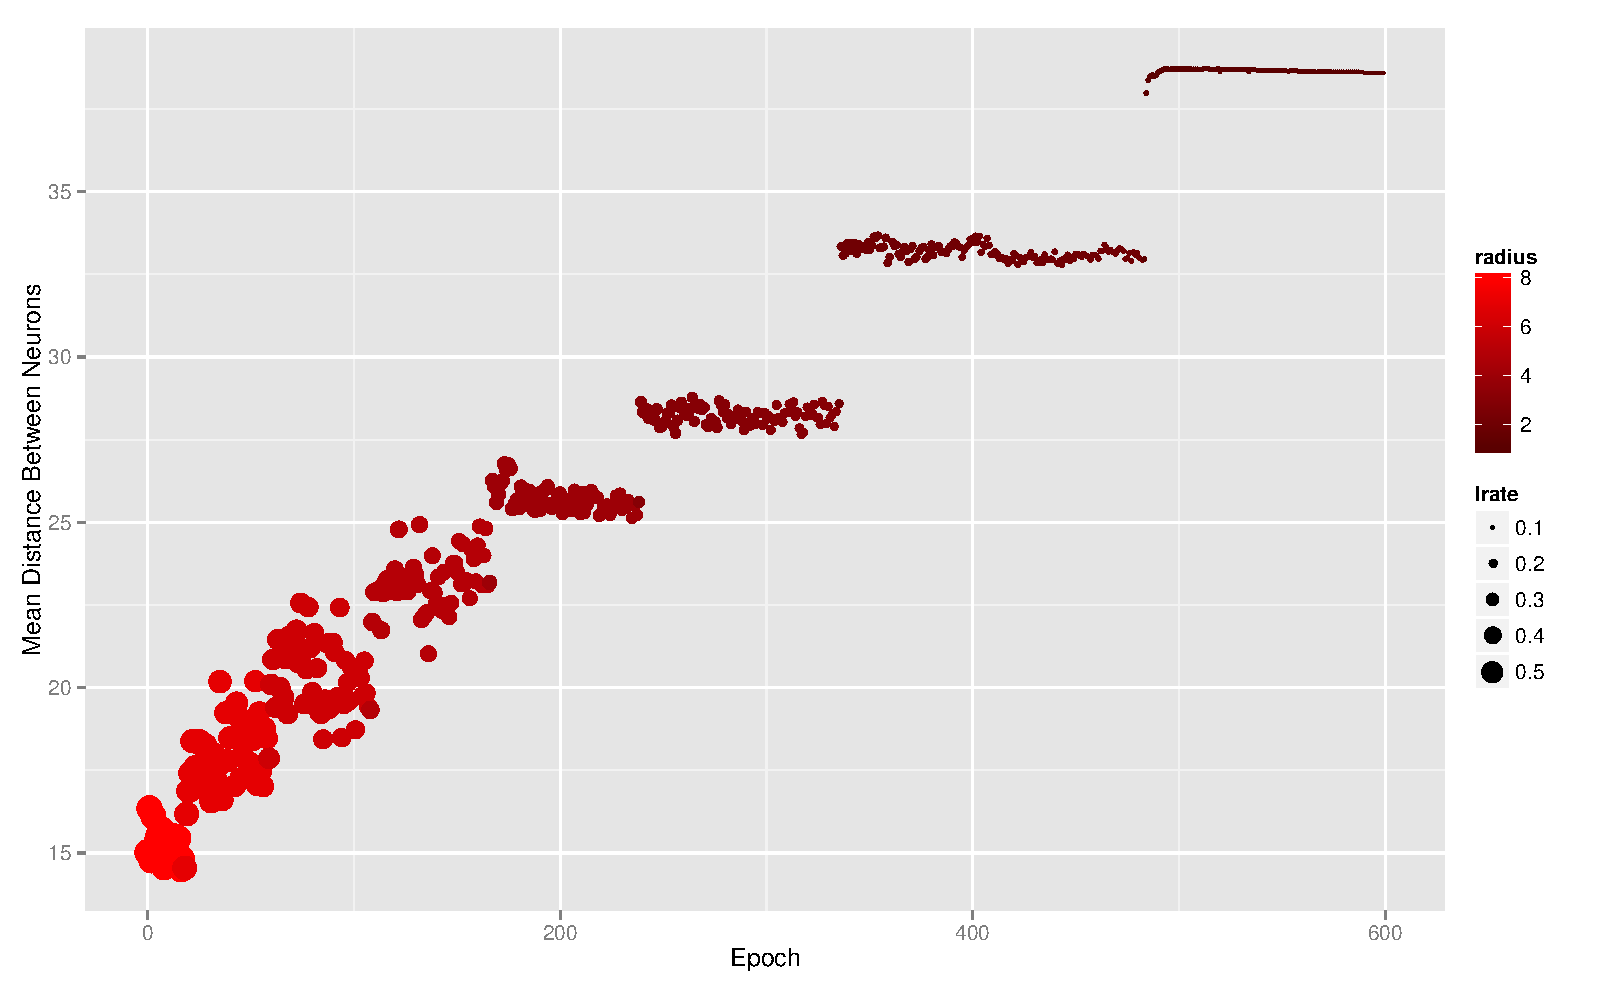
\includegraphics[scale=0.6]{./plots/som/average_distance.pdf}}
  \label{fig:avg_dist}
  \caption{Changes in the average distance between neurons, throughout the SOM training}
\end{figure}

\begin{figure}[htpb]
  \centering
  \subfigure[Output Space]{
\includegraphics[scale=1]{./images/som_training/1_som.pdf}\label{chp3:onesom}}
  \hspace*{0.5cm}
  \subfigure[U-Matrix]{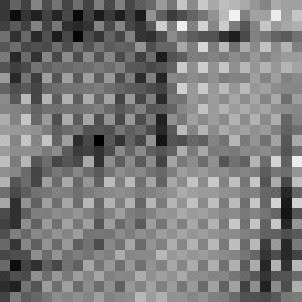
\includegraphics[scale=0.5]{./images/som_training/1_umatrix.pdf}\label{chp3:onematrix}}
  \hspace*{0.5cm}
  \subfigure[Q-Matrix]{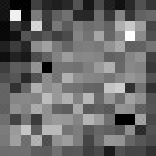
\includegraphics[scale=1]{./images/som_training/1_quantmatrix.pdf}\label{chp3:onetopmat}}
  \hspace*{0.5cm}
  \caption{ SOM state after first epoch of training. Its learning rate is at 0.598, and radius at 8.  }
  \label{fig:}
\end{figure}

\begin{figure}[htpb]
  \centering
  \subfigure[Output Space]{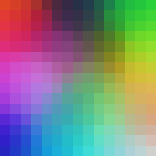
\includegraphics[scale=1]{./images/som_training/2_som.pdf}\label{chp3:onesom}}
  \hspace*{0.5cm}
  \subfigure[U-Matrix]{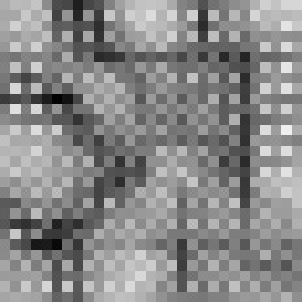
\includegraphics[scale=0.5]{./images/som_training/2_umatrix.pdf}\label{chp3:onematrix}}
  \hspace*{0.5cm}
  \subfigure[Q-Matrix]{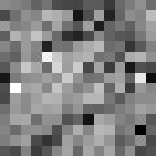
\includegraphics[scale=1]{./images/som_training/2_quantmatrix.pdf}\label{chp3:onetopmat}}
  \hspace*{0.5cm}
  \caption{ SOM state after second epoch of training. Its learning rate is at 0.22, and radius at 3.  }
  \label{fig:}
\end{figure}

\begin{figure}[htpb]
  \centering
  \subfigure[Output Space]{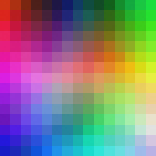
\includegraphics[scale=1]{./images/som_training/3_som.pdf}\label{chp3:onesom}}
  \hspace*{0.5cm}
  \subfigure[U-Matrix]{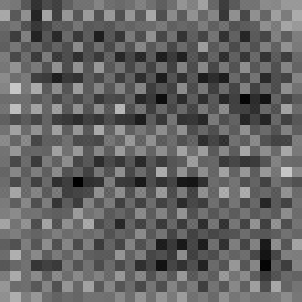
\includegraphics[scale=0.5]{./images/som_training/3_umatrix.pdf}\label{chp3:onematrix}}
  \hspace*{0.5cm}
  \subfigure[Q-Matrix]{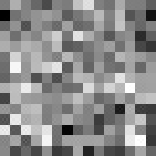
\includegraphics[scale=1]{./images/som_training/3_quantmatrix.pdf}\label{chp3:onetopmat}}
  \hspace*{0.5cm}
  \caption{ SOM state after third epoch of training. Its learning rate is at 0.081, and radius at 1.  }
  \label{fig:}
\end{figure}

\begin{figure}[htpb]
  \centering
  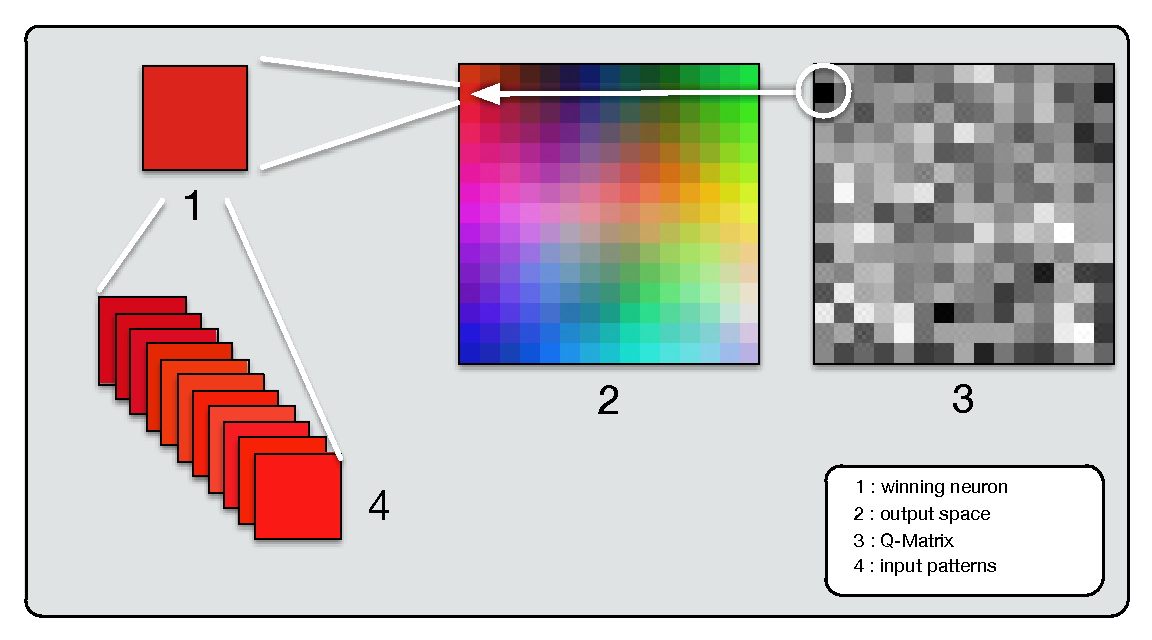
\includegraphics[width=0.8\linewidth]{./images/som_trainned.pdf}
  \caption{Input patterns associated with the neuron with maximum topological error --31. Even though the neuron has the biggest topological error of all neurons, it still has a good representation of the input patterns. The colors in this image are not figurative, and represent the entities at the end of trainning  }
  \label{fig:./images/som_trainned}
\end{figure}

\subsection{Benchmarking}
\label{sub:benchmarking}



\section{Homophilic SOM}
\label{sec:homophilic_som}



\section{Conclusions}
{\color{red} Only these methods are not enough to cluster tweets }

% Ensure that the next chapter starts in a odd page
\cleardoublepage
 
%%%%%% REMOVED STUFF
%\subsection{Topology Preservation} 
%\label{sub:topology_preservation}
%The Self-Organizing Map performs a mapping from the n-dimensional input space into the two dimensional output space and where resides one the most fascinating characteristics, which is that the output map tries to preserve the topology from the input space. This grants the SOM algorithm a way to visualize high-dimensional data that other neural networks or clustering algorithms don't have. Even though this is true, sometimes during training it is not possible to preserve the topology of the network.
%Thus topology preservation can be measured through the Topographic error~\citet{Kiviluoto1996} which is the proportion of all data vectors for which first and second BMUs \footnote{unit that is closest to the winning neuron. BMU Best fitting unit } are not adjacent units.
%In this project the Topographic Error will be calculated for all SOM implementations and VSM usages in order to understand if the representation of the SOM output space is well defined.

 %\begin{itemize}
  %\item show UMatrixes and multiple steps map trainning of the SOM library trainnig
  %\item show metrics for the crawller, tweets per second, users persecond, size of the dump a long the time.
  %\item compare my som library with other som libraries: training velocity with diferent parameters, map after trainned.
  %\item Compare Homophilic-SOM results with non homophilic: UMatrixes, cluster results, Quantization error, jacknife. 
%\end{itemize}
%%\section{Evaluation Metrics} 
%%\label{sec:evaluation_metrics}
%Evaluation of the topic detection on Tweets will be made in two distinct ways. The first way will focus on  binary classification using the precision and recall metrics, and will be described in Subsection~\ref{sub:testing_for_precision_and_recall}. The second way will focus on statistically testing the SOM learning process and the computed trained network. This testing process will be described in Subsection~\ref{sub:cluster_quality_testing}. 

%\section{Testing for Precision and Recall} 
%\label{sec:testing_for_precision_and_recall}
%Precision and Recall are both ways to measure the rate of right guesses made by the trained SOM network, and are defined in the following way:
%\begin{itemize}
  %\item \textbf{Precision:} Fraction of retrieved instances that where relevant 
    %\begin{equation}
  precision = \frac{|{relevant\;documents}\cap{retrieved\;documents}|}{{retrieved\;documents}}
\end{equation} 

  %\item \textbf{Recall:} Fraction of relevant instances that where retrieved
    %\begin{equation}
  recall = \frac{|{relevant\;documents}\cap{retrieved\;documents}|}{{relevant\;documents}} 
\end{equation} 

%\end{itemize}
 
%In order to calculate Precision and Recall we need to have the \emph{relevant documents} and the \emph{retrieved documents}. The \emph{relevant documents} are rather hard to determine because they need to be categorized by humans, which is an expensive task.
